%%
%% Beginning of file 'sample62.tex'
%%
%% Modified 2018 January
%%
%% This is a sample manuscript marked up using the
%% AASTeX v6.2 LaTeX 2e macros.
%%
%% AASTeX is now based on Alexey Vikhlinin's emulateapj.cls 
%% (Copyright 2000-2015).  See the classfile for details.

%% AASTeX requires revtex4-1.cls (http://publish.aps.org/revtex4/) and
%% other external packages (latexsym, graphicx, amssymb, longtable, and epsf).
%% All of these external packages should already be present in the modern TeX 
%% distributions.  If not they can also be obtained at www.ctan.org.

%% The first piece of markup in an AASTeX v6.x document is the \documentclass
%% command. LaTeX will ignore any data that comes before this command. The 
%% documentclass can take an optional argument to modify the output style.
%% The command below calls the preprint style  which will produce a tightly 
%% typeset, one-column, single-spaced document.  It is the default and thus
%% does not need to be explicitly stated.
%%
%%
%% using aastex version 6.2
\documentclass[twocolumn]{aastex62}

%% The default is a single spaced, 10 point font, single spaced article.
%% There are 5 other style options available via an optional argument. They
%% can be invoked like this:
%%
%% \documentclass[argument]{aastex62}
%% 
%% where the layout options are:
%%
%%  twocolumn   : two text columns, 10 point font, single spaced article.
%%                This is the most compact and represent the final published
%%                derived PDF copy of the accepted manuscript from the publisher
%%  manuscript  : one text column, 12 point font, double spaced article.
%%  preprint    : one text column, 12 point font, single spaced article.  
%%  preprint2   : two text columns, 12 point font, single spaced article.
%%  modern      : a stylish, single text column, 12 point font, article with
%% 		  wider left and right margins. This uses the Daniel
%% 		  Foreman-Mackey and David Hogg design.
%%  RNAAS       : Preferred style for Research Notes which are by design 
%%                lacking an abstract and brief. DO NOT use \begin{abstract}
%%                and \end{abstract} with this style.
%%
%% Note that you can submit to the AAS Journals in any of these 6 styles.
%%
%% There are other optional arguments one can envoke to allow other stylistic
%% actions. The available options are:
%%
%%  astrosymb    : Loads Astrosymb font and define \astrocommands. 
%%  tighten      : Makes baselineskip slightly smaller, only works with 
%%                 the twocolumn substyle.
%%  times        : uses times font instead of the default
%%  linenumbers  : turn on lineno package.
%%  trackchanges : required to see the revision mark up and print its output
%%  longauthor   : Do not use the more compressed footnote style (default) for 
%%                 the author/collaboration/affiliations. Instead print all
%%                 affiliation information after each name. Creates a much
%%                 long author list but may be desirable for short author papers
%%
%% these can be used in any combination, e.g.
%%
%% \documentclass[twocolumn,linenumbers,trackchanges]{aastex62}
%%
%% AASTeX v6.* now includes \hyperref support. While we have built in specific
%% defaults into the classfile you can manually override them with the
%% \hypersetup command. For example,
%%
%%\hypersetup{linkcolor=red,citecolor=green,filecolor=cyan,urlcolor=magenta}
%%
%% will change the color of the internal links to red, the links to the
%% bibliography to green, the file links to cyan, and the external links to
%% magenta. Additional information on \hyperref options can be found here:
%% https://www.tug.org/applications/hyperref/manual.html#x1-40003
%%
%% If you want to create your own macros, you can do so
%% using \newcommand. Your macros should appear before
%% the \begin{document} command.
%%
\usepackage{color}

\newcommand{\vdag}{(v)^\dagger}
\newcommand\aastex{AAS\TeX}
\newcommand\latex{La\TeX}
\newcommand{\colorred}[1]{\color{red}#1\color{black}\hspace{0.5mm}}

\setlength{\tabcolsep}{2pt}

%% Reintroduced the \received and \accepted commands from AASTeX v5.2
% \received{January 1, 2018}
% \revised{January 7, 2018}
% \accepted{\today}
%% Command to document which AAS Journal the manuscript was submitted to.
%% Adds "Submitted to " the argument.
% \submitjournal{ApJ}

%% Mark up commands to limit the number of authors on the front page.
%% Note that in AASTeX v6.2 a \collaboration call (see below) counts as
%% an author in this case.
%
%\AuthorCollaborationLimit=3
%
%% Will only show Schwarz, Muench and "the AAS Journals Data Scientist 
%% collaboration" on the front page of this example manuscript.
%%
%% Note that all of the author will be shown in the published article.
%% This feature is meant to be used prior to acceptance to make the
%% front end of a long author article more manageable. Please do not use
%% this functionality for manuscripts with less than 20 authors. Conversely,
%% please do use this when the number of authors exceeds 40.
%%
%% Use \allauthors at the manuscript end to show the full author list.
%% This command should only be used with \AuthorCollaborationLimit is used.

%% The following command can be used to set the latex table counters.  It
%% is needed in this document because it uses a mix of latex tabular and
%% AASTeX deluxetables.  In general it should not be needed.
%\setcounter{table}{1}

%%%%%%%%%%%%%%%%%%%%%%%%%%%%%%%%%%%%%%%%%%%%%%%%%%%%%%%%%%%%%%%%%%%%%%%%%%%%%%%%
%%
%% The following section outlines numerous optional output that
%% can be displayed in the front matter or as running meta-data.
%%
%% If you wish, you may supply running head information, although
%% this information may be modified by the editorial offices.
\shorttitle{Effects of Primordial Binaries on Evolutionary}
\shortauthors{Thomas M. Boudreaux et al.}
%%
%% You can add a light gray and diagonal water-mark to the first page 
%% with this command:
% \watermark{text}
%% where "text", e.g. DRAFT, is the text to appear.  If the text is 
%% long you can control the water-mark size with:
%  \setwatermarkfontsize{dimension}
%% where dimension is any recognized LaTeX dimension, e.g. pt, in, etc.
%%
%%%%%%%%%%%%%%%%%%%%%%%%%%%%%%%%%%%%%%%%%%%%%%%%%%%%%%%%%%%%%%%%%%%%%%%%%%%%%%%%

%% This is the end of the preamble.  Indicate the beginning of the
%% manuscript itself with \begin{document}.

\begin{document}

% REU: The title is the single most important element of the paper, because it is the part
% most widely used for literature searches.  Make sure that your title is about WHAT
% you did, and not solely focused on HOW you did it.  The methods you used are
% secondary to what you accomplished.  In other words, put your science first.

\title{Effects of Primordial Binary Fraction on Globular Cluster Evolution}

%% LaTeX will automatically break titles if they run longer than
%% one line. However, you may use \\ to force a line break if
%% you desire. In v6.2 you can include a footnote in the title.

%% A significant change from earlier AASTEX versions is in the structure for 
%% calling author and affilations. The change was necessary to implement 
%% autoindexing of affilations which prior was a manual process that could 
%% easily be tedious in large author manuscripts.
%%
%% The \author command is the same as before except it now takes an optional
%% arguement which is the 16 digit ORCID. The syntax is:
%% \author[xxxx-xxxx-xxxx-xxxx]{Author Name}
%%
%% This will hyperlink the author name to the author's ORCID page. Note that
%% during compilation, LaTeX will do some limited checking of the format of
%% the ID to make sure it is valid.
%%
%% Use \affiliation for affiliation information. The old \affil is now aliased
%% to \affiliation. AASTeX v6.2 will automatically index these in the header.
%% When a duplicate is found its index will be the same as its previous entry.
%%
%% Note that \altaffilmark and \altaffiltext have been removed and thus 
%% can not be used to document secondary affiliations. If they are used latex
%% will issue a specific error message and quit. Please use multiple 
%% \affiliation calls for to document more than one affiliation.
%%
%% The new \altaffiliation can be used to indicate some secondary information
%% such as fellowships. This command produces a non-numeric footnote that is
%% set away from the numeric \affiliation footnotes.  NOTE that if an
%% \altaffiliation command is used it must come BEFORE the \affiliation call,
%% right after the \author command, in order to place the footnotes in
%% the proper location.
%%
%% Use \email to set provide email addresses. Each \email will appear on its
%% own line so you can put multiple email address in one \email call. A new
%% \correspondingauthor command is available in V6.2 to identify the
%% corresponding author of the manuscript. It is the author's responsibility
%% to make sure this name is also in the author list.
%%
%% While authors can be grouped inside the same \author and \affiliation
%% commands it is better to have a single author for each. This allows for
%% one to exploit all the new benefits and should make book-keeping easier.
%%
%% If done correctly the peer review system will be able to
%% automatically put the author and affiliation information from the manuscript
%% and save the corresponding author the trouble of entering it by hand.

\correspondingauthor{Thomas M.\ Boudreaux}
\email{thomas@boudreauxmail.com}

% REU: This shows how to format the names.  Use your full name, spelled out the way
% you want it to appear in the literature.  The 16-digit number inside the [] should
% be replaced with your ORCID.  If you don't have one, you should sign up for one,
% and put that number here and in all your future papers.  
% For your affiliation, use your home institution and address, not the CfA.
% Your advisor will be able to tell you whose names appear here.

\author[0000-0002-2600-7513]{Thomas M.\ Boudreaux}
\affil{High Point University, \\One University Pkwy, \\High Point, NC, 27268}

\author{Idan Ginsburg}
\affiliation{Harvard-Smithsonian Center for Astrophysics \\
60 Garden St. \\
Cambridge, MA 02138, USA}
% \collaboration{(AAS Journals Data Scientists collaboration)}

% \author{Advisor 2.\ Name}
% \affiliation{National Radio Astronomy Observatory}
% \affiliation{AAS Journals Associate Editor-in-Chief}
%  %\nocollaboration

% \author{Amy Hendrickson}
% \affiliation{TeXnology Inc.}
% % \collaboration{(LaTeX collaboration)}

% \author{Julie Steffen}
% \affiliation{AAS Director of Publishing}
% \affiliation{American Astronomical Society \\
% 2000 Florida Ave., NW, Suite 300 \\
% Washington, DC 20009-1231, USA}

% \author{Jeff Lewandowski}
% \affiliation{IOP Senior Publisher for the AAS Journals}
% \affiliation{IOP Publishing, Washington, DC 20005}

%% AASTeX 6.2 has the new \collaboration and \nocollaboration commands to
%% provide the collaboration status of a group of authors. These commands 
%% can be used either before or after the list of corresponding authors. The
%% argument for \collaboration is the collaboration identifier. Authors are
%% encouraged to surround collaboration identifiers with ()s. The 
%% \nocollaboration command takes no argument and exists to indicate that
%% the nearby authors are not part of surrounding collaborations.

% Mark off the abstract in the ``abstract'' environment. 
\begin{abstract}

ABSTRACT HERE --- NOTE this is a very early rough draft. NB: Any text in red is text which either needs to be filled in, or will almost certainly change; however, other text very will may change as the project progresses.

\end{abstract}

%% Keywords should appear after the \end{abstract} command. 
%% See the online documentation for the full list of available subject
%% keywords and the rules for their use.
\keywords{editorials, notices --- 
miscellaneous --- catalogs --- surveys}

%% From the front matter, we move on to the body of the paper.
%% Sections are demarcated by \section and \subsection, respectively.
%% Observe the use of the LaTeX \label
%% command after the \subsection to give a symbolic KEY to the
%% subsection for cross-referencing in a \ref command.
%% You can use LaTeX's \ref and \label commands to keep track of
%% cross-references to sections, equations, tables, and figures.
%% That way, if you change the order of any elements, LaTeX will
%% automatically renumber them.
%%
%% We recommend that authors also use the natbib \citep
%% and \citet commands to identify citations.  The citations are
%% tied to the reference list via symbolic KEYs. The KEY corresponds
%% to the KEY in the \bibitem in the reference list below. 

\section{Introduction} \label{sec:intro}

Globular clusters (GCs) are among the oldest observable objects in the universe \citep{Pen11}. Characterized by their high densities --- with typical half--light radii in the range of 3 ly, and masses ranging from $10^{4}$ -- $ 10^{5} $ M$_{\odot}$ \citep{Bro06}. GCs provide a unique way to probe stellar evolution \colorred{[CITATION]}, galaxy formation models \citep{Boy18, Kra05}, and dark matter halo structure \citep{Hud18}. Additionally, some important questions surrounding globular clusters remain open. The second parameter problem \citep{Nor83} --- which arose with the understanding that, while cluster metallicity played an important role in shaping horizontal branch structure, metallicity is not alone sufficient to explain these morphological differences \citep{Dot13} --- lacks a widely accepted solution. Moreover, the evolutionary channels followed by GCs as they progress towards open clusters are not fully understood \citep{Mad17}. Expansion and evaporation are two important factors governing this evolution \citep{Fal01}; however some initial conditions of the cluster, which may affect both evaporation and core radius expansion rates, remain relatively unconstrained.

Understanding the evaporation and expansion history of GCs can shed light on both galactic potential in which the cluster lives, and where the cluster formed in that potential \citep{Ren17}. \citet{Wil03} and \citet{Gon05} presented early evidence --- via numeric studies --- that the primordial binary fraction of a cluster may influence a clusters core radius expansion rate, with results indicating that a direct proportionality between binary fraction and expansion rates may exist. Further, \citet{Lan07} provided empirical evidence, through a study of blue straggler stars (BSS) --- effective indicators of binarity --- in M5, that collisional binaries may increase evaporation rates. However, even with these past studies, there has yet to be a firm quantitative relation established between the primordial binary fraction of a cluster and its evolutionary rates. Here we attempt to develop such a relation.

To find a quantitative relation between the binarity of a cluster and its evolutionary rates, multiple GCs within galactic potentials are first generated using McLuster\footnote{https://github.com/ahwkuepper/mcluster} \citep{Kup11}. Only the primordial binary fraction is modified between simulations. These are then numerically integrated over approximatly 12.9 Gyr using NBody6++GPU\footnote{https://github.com/nbodyx/Nbody6ppGPU} \citep{Wan15}.  Core radius expansion and mass evaporate rates across the different primordial binary fraction GCs are then fit \colorred{[or not fit if no relation is found]} to a \colorred{[SOME MODEL]}.  We find blah...\colorred{ [BASIC OVERVIEW OF RESULTS] Basic overview of results Lorem ipsum dolor sit amet, consectetur adipiscing elit, sed do eiusmod tempor incididunt ut labore et dolore magna aliqua. Ut enim ad minim veniam, quis nostrud exercitation ullamco laboris nisi ut aliquip ex ea commodo consequat. Duis aute irure dolor in reprehenderit in voluptate velit esse cillum dolore eu fugiat nulla pariatur. Excepteur sint occaecat cupidatat non proident, sunt in culpa qui officia deserunt mollit anim id est laborum.}

This paper is organized as follows: in Section 2 a description of the simulation initial conditions and run parameters is provided. Section 3 details the analysis conducted on the output data from the simulation. The implications of these results are discussed in section 4, and finally a brief summary is presented in section 5.

\section{NBody Simulation} \label{sec:nbody} 
Direct numerical integration of the NBody problem, while conceptually simple is, in practice, difficult to realize. Naive implementations of such code tend to loose accuracy over large time scales. Nbody6++GPU, an offshoot of Nbody6 \citep{Aar99}, has been shown to maintain high levels of floating point accuracy over giga--year timescales \colorred{[CITATION]}. Additionally, Nbody6++GPU extends the original Nbody6 code both for use with compute cores on modern graphical Processing Units (GPUs), and for use with new CPU instructions set extensions such as the x86 based Advanced Vector Extensions (AVX). These additions make NBody6++GPU well suited for running multiple, \colorred{large [which scale term?] scale}  simulations on highly parrelalized computer systems.

Using McLuster we generate \colorred{1} cluster following the King density profile \citep{Kin62} (Figure \ref{fig:init_distribution}). Macroscale parameters used in the generation of this cluster can be found in Table \ref{tab:macInput}. The full set of input parameters for this cluster are copied and modified such that result in \colorred{10} clusters, which only vary in their primordial binary fraction. We allow the primordial binary fractions to range from \colorred{0.0} to \colorred{1.0} in increments of \colorred{0.1}. These clusters are then placed within a Hernquist \citep{Her90}, Miyamoto Disk \citep{Miy75}, and Dark Matter halo potential (McLuster input parameter t=3). We use a high performance computer cluster and NBody6++GPU to directly numerically integrate each of the \colorred{10} clusters over approximately one Hubble time. During each simulation snapshots of both overall cluster parameters (center of mass location, cluster velocity, etc...) and parameters for each component of the cluster are written to disk every \colorred{1.2 Myr} of simulation time (\colorred{1} Nbody6 time unit).

\begin{table}
    \centering
    \begin{tabular}{c| c c c}
        \hline
        \hline
        Name & Description & Value & Unit \\
        \hline
        $N$ & Number of particles & 1000 \\
        $M$ & Total cluster mass & 516.6 & M$_{\odot}$ \\
        $M_{max}$ & Maximum star mass & 50 & M$_{\odot}$ \\
        $M_{min}$ & Minimum star mass & [TBFI] & M$_{\odot}$ \\
        $F_{B}$ & Primordial Binary Fraction & 0-1.0 \\
        $W_{0}$ & [\colorred{King Parameter}] & 2.0 \\
        
    \end{tabular}
    \caption{Macroscopic Parameters of Cluster...To be filled in as these values are known}
    \label{tab:macInput}
\end{table}

This paragraph is a place holder to help with spacing, which gets all messed up when there is no text here. General input parameters are shown in Table \ref{tab:macInput}, with the full input file shown in Appendix \ref{apx:params}. The initial distribution of mass can be see in Figure \ref{fig:init_distribution} [STUFF NOT YET DONE]. [FILL IN SPECIFIC DETAILS ABOUT SIMULATIONS] \colorred{Lorem ipsum dolor sit amet, consectetur adipiscing elit, sed do eiusmod tempor incididunt ut labore et dolore magna aliqua. Ut enim ad minim veniam, quis nostrud exercitation ullamco laboris nisi ut aliquip ex ea commodo consequat. Duis aute irure dolor in reprehenderit in voluptate velit esse cillum dolore eu fugiat nulla pariatur. Excepteur sint occaecat cupidatat non proident, sunt in culpa qui officia deserunt mollit anim id est laborum.}

\begin{figure}
    \centering
    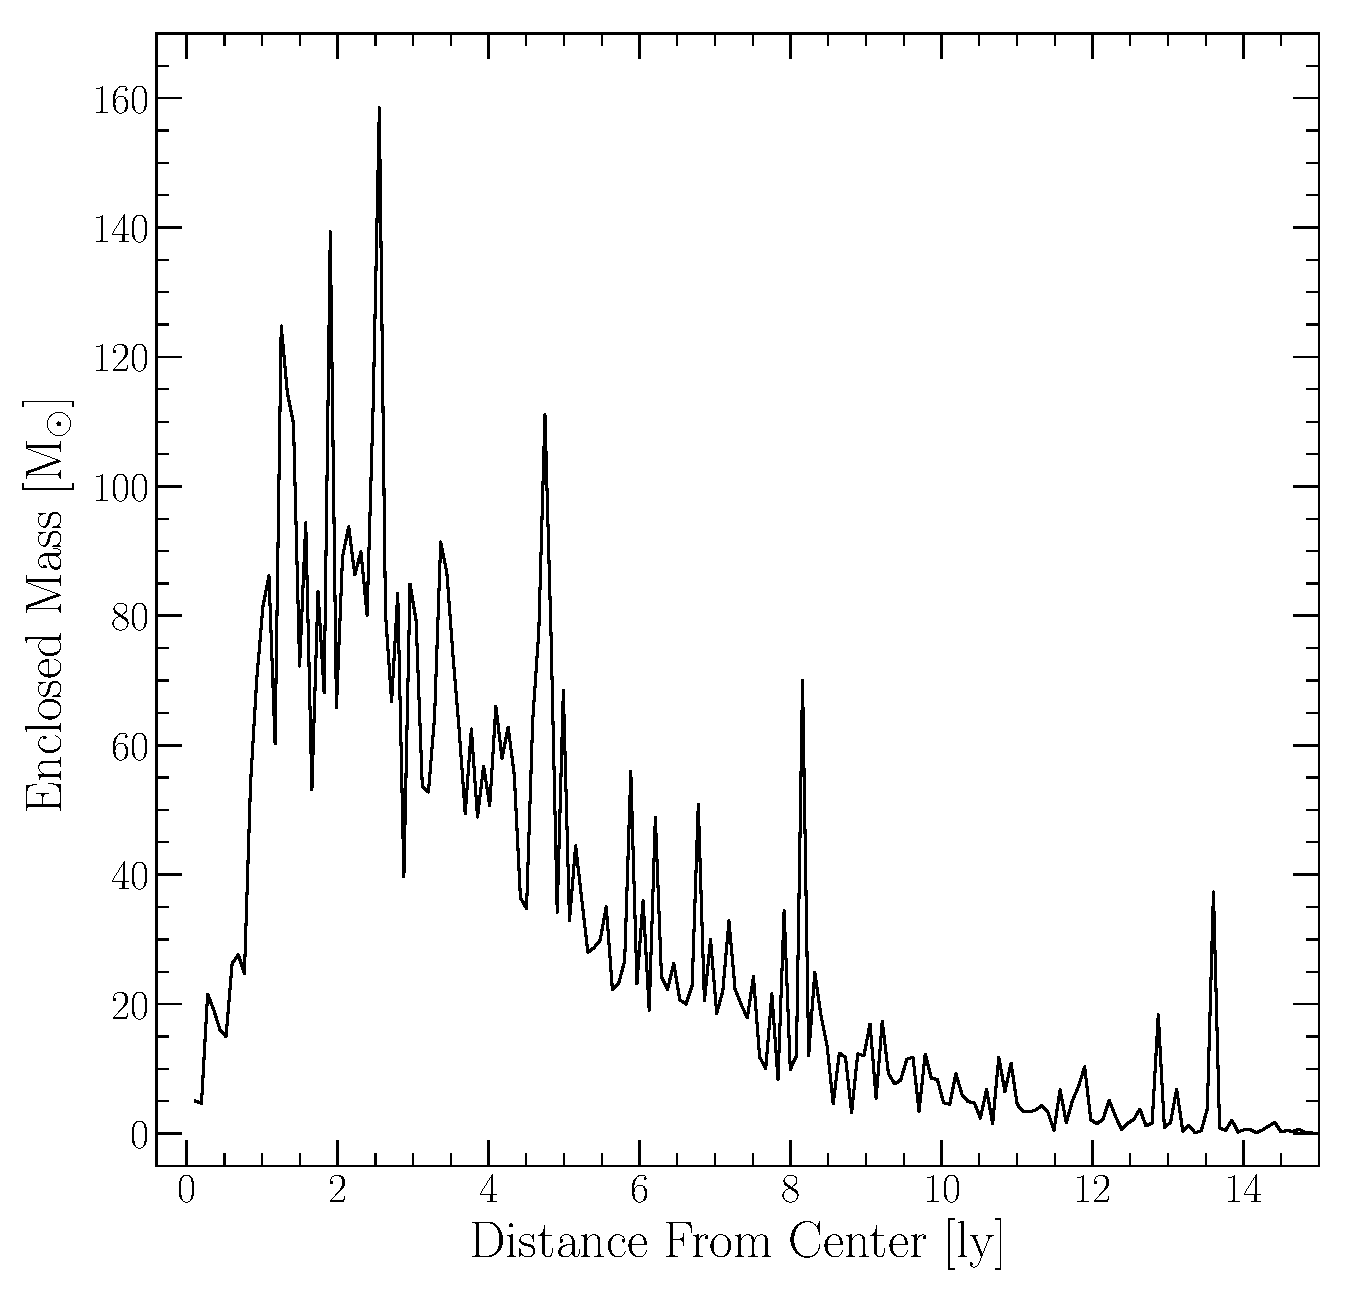
\includegraphics[scale=0.32]{Figures/EnclosedMass.eps}
    \caption{Initial radial mass distribution. Shells 0.07 ly wide are built up from the origin outwards, each point on the graph is the sum of the mass enclosed within a shell.}
    \label{fig:init_distribution}
\end{figure}

\section{Analysis}\label{sec:analysis}
Temporary Figure seen in Figure \ref{fig:HR}. Core Radius expansion is shown in Figure \ref{fig:RCexpand}. Section to be filled in when simulation results are in.
\begin{figure}
    \centering
    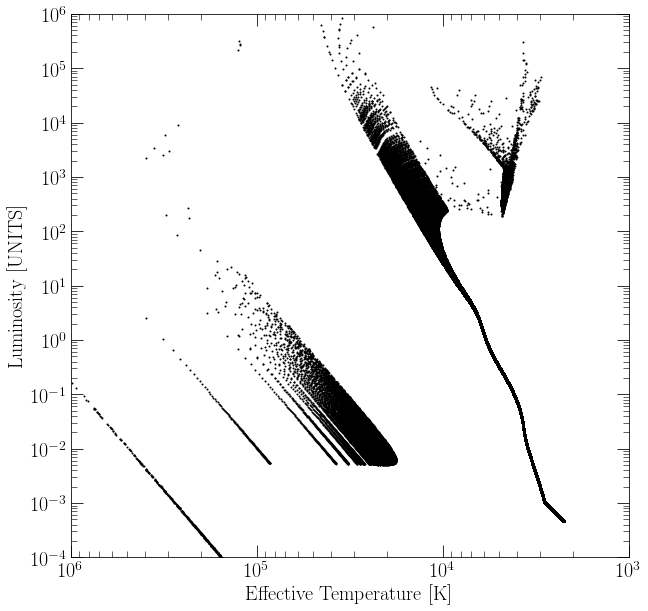
\includegraphics[scale=0.35]{Figures/10000BasicEvolutionHR.png}
    \caption{Luminosity--Temperature Diagram Showing evolution during first 200 snapshots (280 Myr) of simulation. Parameters here, metallicity, age, ... note high mass turn off ... This figure and caption act as place holders.}
    \label{fig:HR}
\end{figure}

\begin{figure}
    \centering
    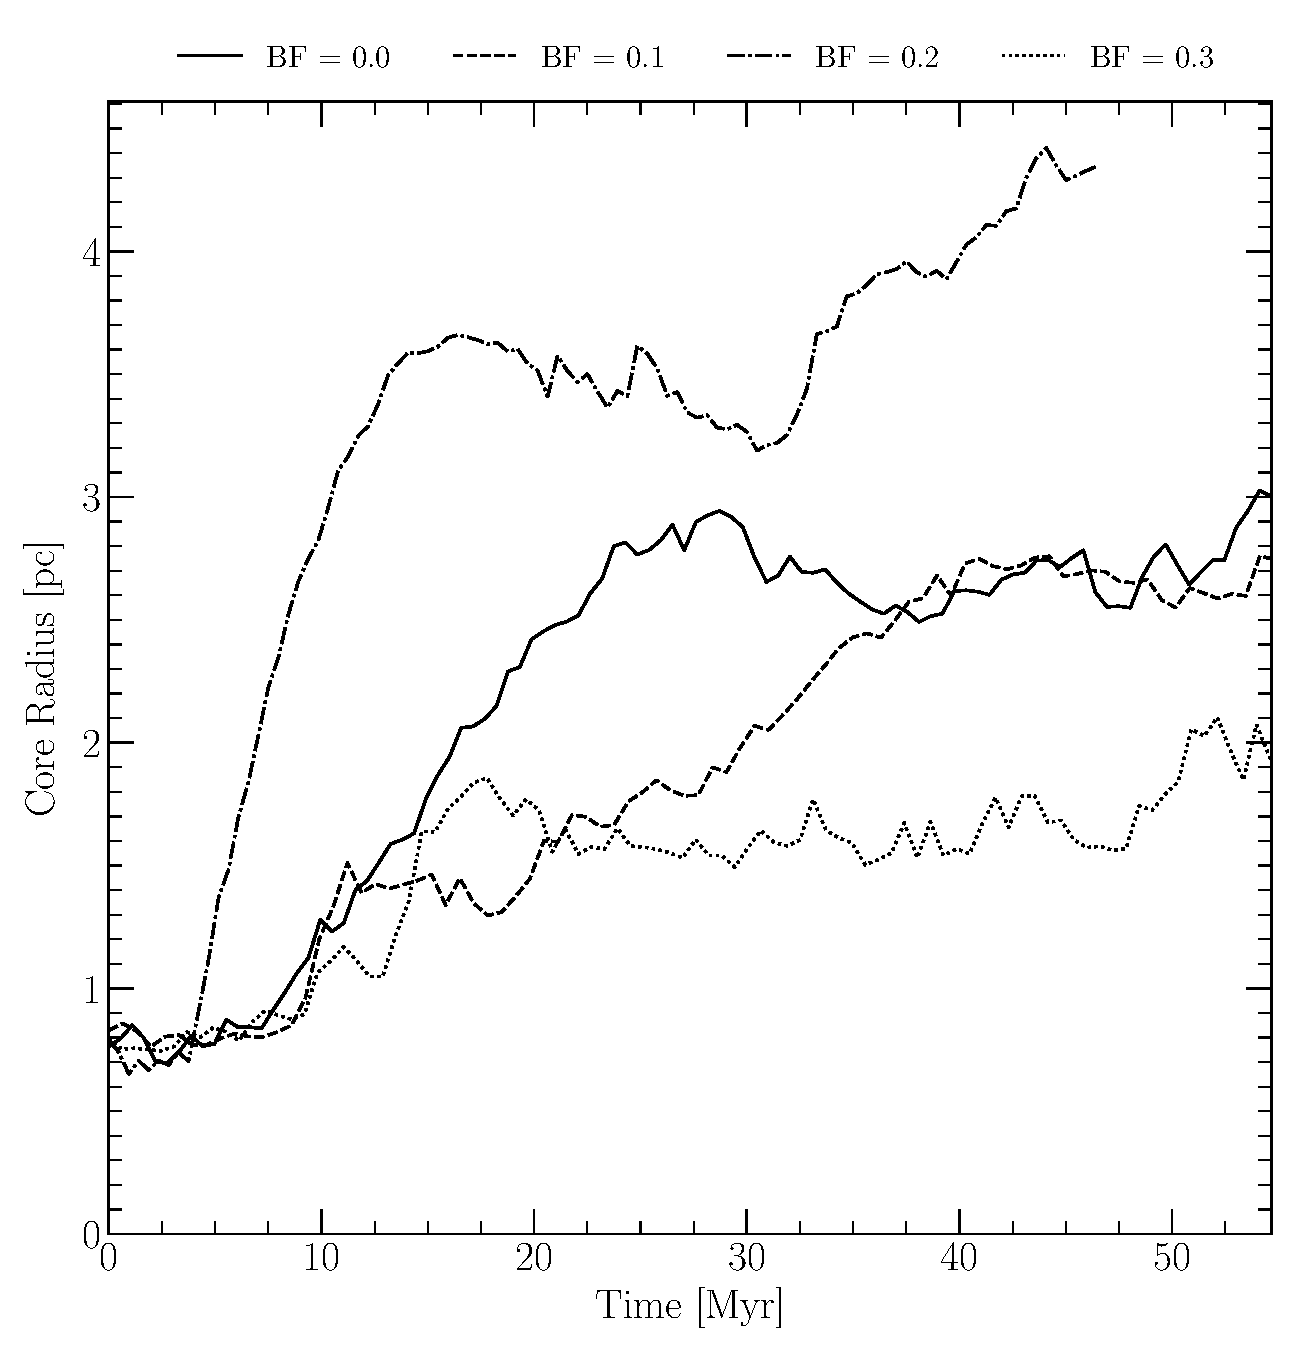
\includegraphics[scale=0.35]{Figures/core_radius_expansion.eps}
    \caption{Core radius expansion of [TEMPORARY EXPERIMENTATION] clusters with different primordial binary fractions. Note that this temporary figure is meaningless as more than the primordial binary fraction was changed between runs.}
    \label{fig:RCexpand}
\end{figure}

\subsection{Core Radius Expansion}

\subsection{Mass Evaporation}

\section{Discussion}\label{sec:disscussion}

\section{Conclusion}\label{sec:conclusion}

\section{Acknowledgements}\label{sec:acknowledgements}



\appendix

\section{Simulation Initial Conditions}\label{apx:params}

\begin{table}[ht]
    \centering
    \begin{tabular}{c | l l l l l l l l l l}
        \hline
        \hline
        \textbf{nbody6.F} & KSTART & TCOMP & TCRITp & isernb & iserreg & iserks \\
        \hline
        \textbf{input.F} & N & NFIX & NCRIT & NRAND & NNBOPT & NRUN \\
        & ETAI & ETAR & RSO & DTADJ & DELTAT & TCRIT & QE & RBAR & ZMBAR \\
        & KZ(1) & KZ(2) & KZ(3) & KZ(4) & KZ(5) & KZ(6) & KZ(7) & KZ(8) & KZ(9) & KZ(10) \\
        & KZ(11) & KZ(12) & KZ(13) & KZ(14) & KZ(15) & KZ(16) & KZ(17) & KZ(18) & KZ(19) & KZ(20) \\
        & KZ(21) & KZ(22) & KZ(23) & KZ(24) & KZ(25) & KZ(26) & KZ(27) & KZ(28) & KZ(29) & KZ(30) \\
        & KZ(31) & KZ(32) & KZ(33) & KZ(34) & KZ(35) & KZ(36) & KZ(37) & KZ(38) & KZ(39) & KZ(40) \\
        & KZ(41) & KZ(42) & KZ(43) & KZ(44) & KZ(45) & KZ(46) & KZ(47) & KZ(48) & KZ(49) & KZ(50) \\
        & DTMIN & RMIN & ETAU & ECLOSE & GMIN & GMAX & SMAX \\
        \hline
        \textbf{data.F} & ALPHA & BODY1 & BODYN & NBINO & NHIO & ZMET & EPOCHO & DTPLOT \\
        \hline
        \textbf{setup.F} & APO & ECC & N2 & SCALE & & & & & &  (KZ(5)=2) \\
        & APO & ECC & SCALE & & & & & & & (KZ(5)=3) \\
        & APO & ECC & SCALE & & & & & & &  (KZ(5)=3) \\
        & SEMI & ECC & M1 & M2 & & & & & &  (KZ(5)=4) \\
        & ZMH & RCUT & & & & & & &  & (KZ(5)=6\&KZ(24)$<$0) \\
        \hline
        \textbf{scale.F} & Q & VXROT & VZROT & RTIDE \\
        \hline
        \textbf{xtrn10.F} & GMG & RGO & & & & & & & &   (KZ(14)=2) \\
        & GMG & DISK & A & B & VCIRC & RCIRC & GMB & AR & GAM \\
        & RG[1:3] & VG[1:3] & & & & & & & &   (KZ(14)=3) \\
        & MP & AP & MPDOT & TDELAY & & & & & &  (KZ(14)=3$||$KZ(14)=4) \\
        \hline
        \textbf{binpop.F} & SEMI & ECC & RATIO & RANGE & NSKIP & IDORM & & & & (KZ(8)=1$||$KZ(8)$>$4) \\
        \hline
        \textbf{hipop.F} & SEMI & ECC & RATIO & RANGE & & & & & & (KZ(8)$>$0\&KZ(18)$>$1) \\
        \hline
        \textbf{imbhinit.F} & MMBH & XBH(1) & XBH(2) & XBH(3) & VBH(1) & VBH(2) & VBH(3) & DTBH & & (KZ(24)=1) \\
        \hline
        \textbf{cloud0.F} & NCL & RB2 & VCL & SIGMA & CLM & RCL2 & & & & (KZ(13)$>$0) \\
        \hline
    \end{tabular}
    \caption{Table to be populated by initial conditions when those are available. Currently used as reference for parameter locations in input grid.}
    \label{tab:inputref}
\end{table}


\bibliographystyle{aasjournal}
\bibliography{ms}

\end{document}

